\makeatletter\def\input@path{{minimus}{standalone-silicon}}\makeatother

\documentclass{standalone-silicon}

\usepackage{minimus-text}
\usepackage{minimus-math}
\usepackage{minimus-tikz}

\begin{document}
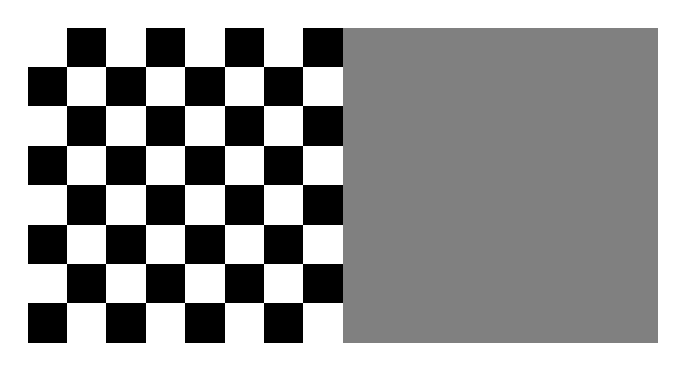
\begin{tikzpicture}

\def\step{0.5}
\foreach \x in {0,\fpeval{\step*2},...,3.99}
{
    \foreach \y in {0,\fpeval{\step*2},...,3.99}
    {
        \fill[black] (\x,\y) rectangle (\fpeval{\x+\step},\fpeval{\y+\step});
        \fill[black] (\fpeval{\x+\step},\fpeval{\y+\step}) rectangle (\fpeval{\x+2*\step},\fpeval{\y+2*\step});
    }
}

\fill[white!\fpeval{100*0.5}!black] (4,0) rectangle (8,4);

\end{tikzpicture}
\end{document}